\subsection{Implementación de firmware}

\subsubsection{Lógica a nivel general}


El SAL/T resulta un sistema bastante complejo por la cantidad de entradas y variantes de comportamiento que considera para determinar su modo de operación y la activación de las señales críticas que resulta el componente de salida más relevante del sistema que le da propósito al SAL/T. La lógica de alto nivel que se puede considerar para el SAL/T se visualiza en la figura \ref{fig:logica_firmware}.  \\


Al comienzo, se inicializan todos los periféricos, las comunicaciones, los módulos y la memoria que forman parte del sistema. Por su lado, el ESP32 va a inicializarse y comunicarse con el servidor MQTT a través de alguna de las redes Wi-Fi que tenga configurado, para suscribirse a la recepción de comandos y poder reportar el estado y registro de eventos del sistema de manera remota. \\

Luego, se leen las entradas del sistema. Por un lado, el sistema lee el estado de las llaves de activación de modo aislado limitado y total, y los comandos remotos para determinar el modo de operación del SAL/T. Por otro lado, se leen las entradas del estado de los SIS, la ubicación GPS, la velocidad que puede ser obtenida por cualquiera de sus fuentes de medición siguiendo la prioridad de Hasler Tesloc 1500, luego el generador de impulsos ópticos y luego la señal GPS. \\ 

Una vez que el sistema tiene el dato de todas las entradas, va a mostrar a través del panel frontal y registrar a través del almacenamiento interno y remoto, cualquier estado o cambio relevante del sistema. \\ 

Luego, se determina cuál debe ser el modo de operación del SAL/T basado en el primer grupo de entradas mencionado, y se activan las rutinas de entrada en cada modo. \\

Finalmente, con el modo de operación ya configurado y el resto de las entradas, se determina los valores que deben tomar las salidas de señales críticas como el corte de tracción, freno de emergencia o bypass de los SIS. Al finalizar, se vuelve al comienzo de lectura de entradas y se mantiene funcionando esta lógica de manera general en todo momento. 


\begin{figure}[H]
    \centering
    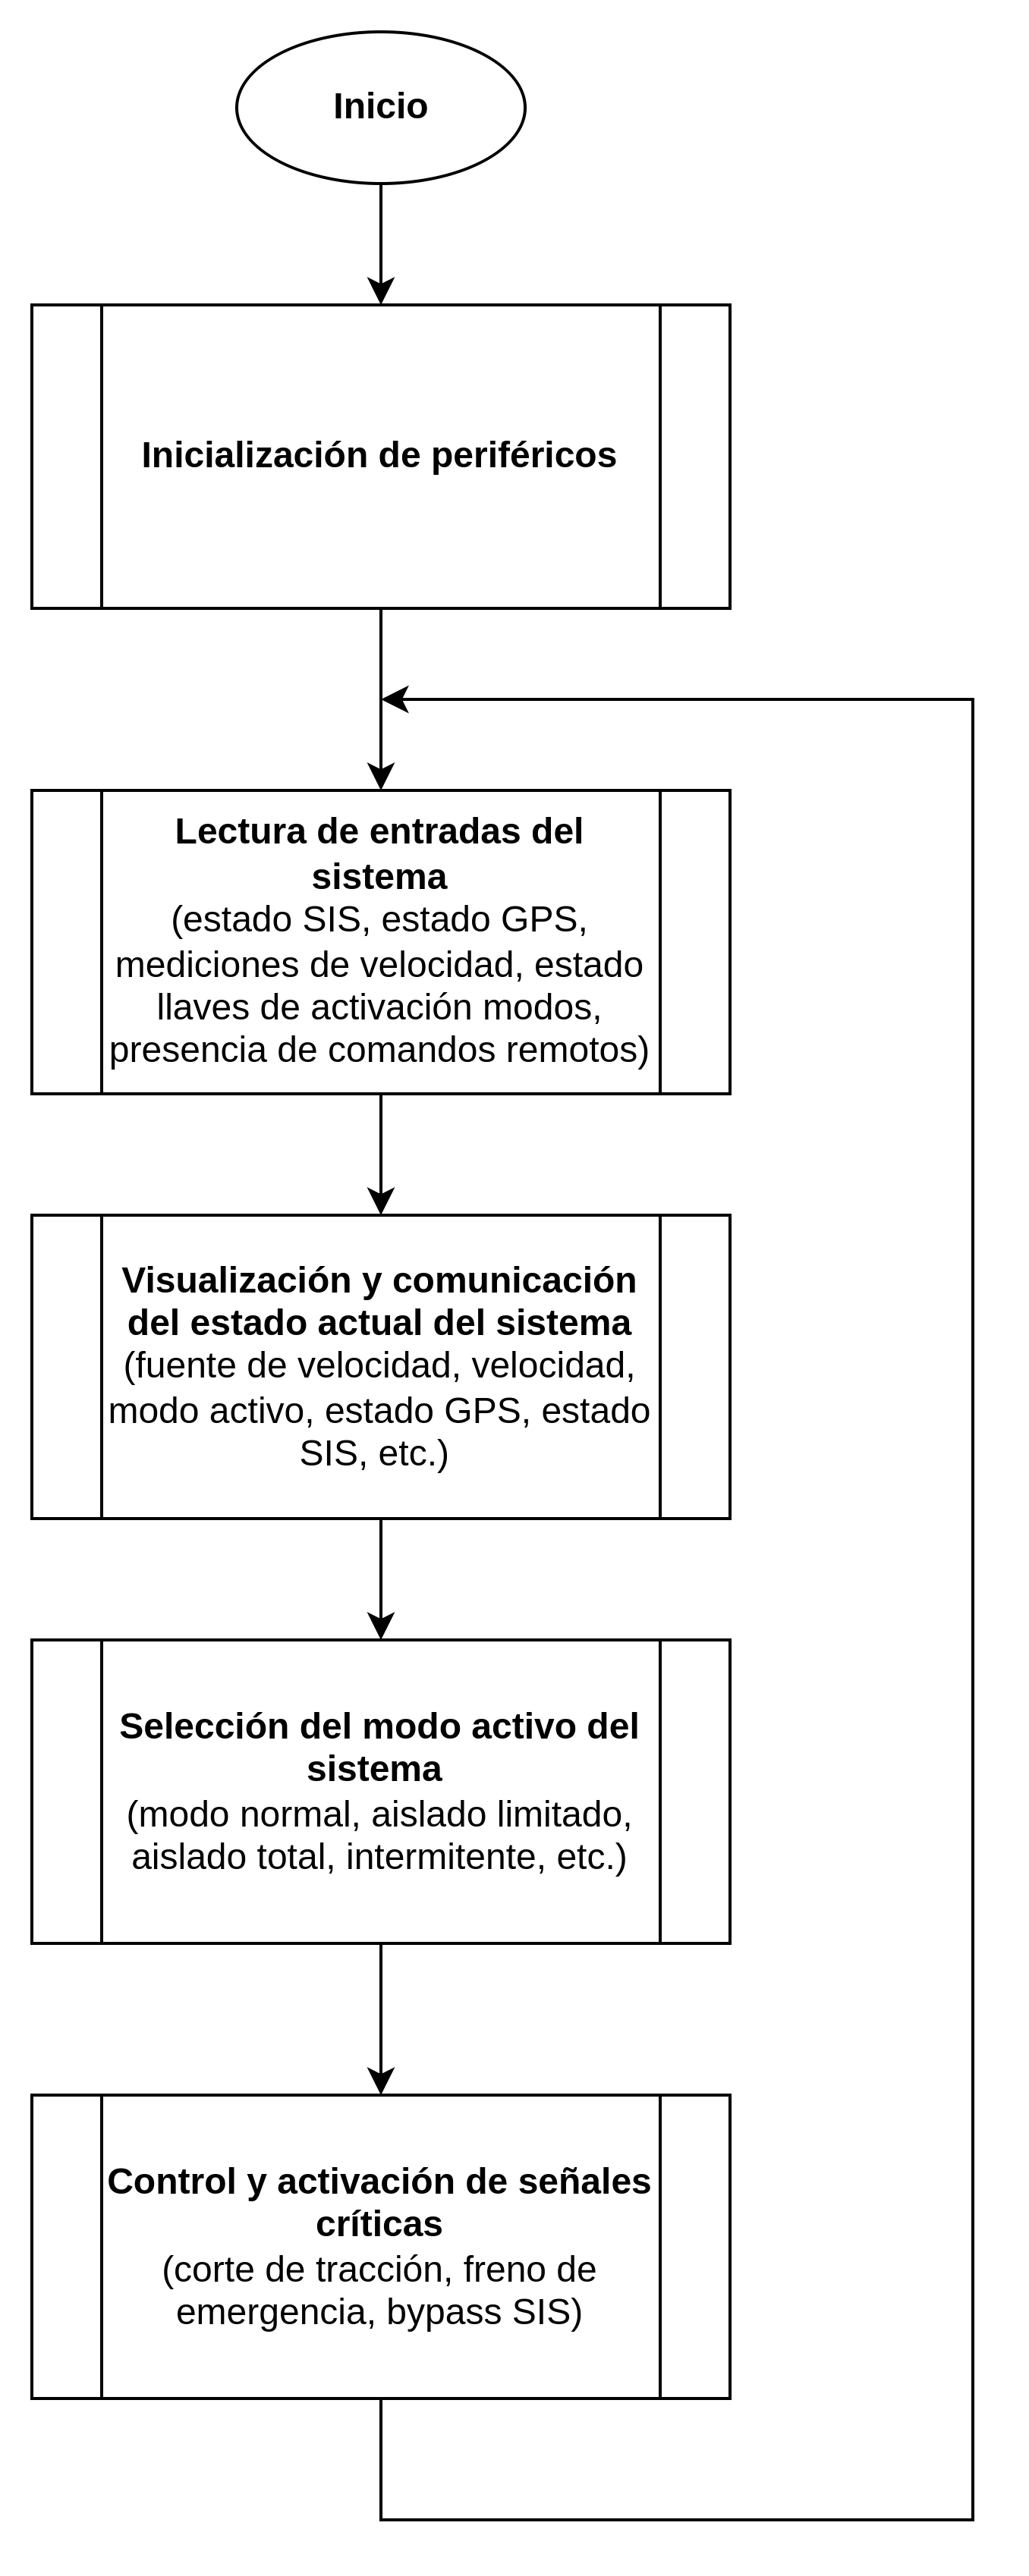
\includegraphics[scale = 0.6]{img/logica_firmware.png}    
    \caption{Lógica general del firmware del SAL/T}
    \label{fig:logica_firmware}
\end{figure}    




En la figura \ref{fig:modos_salt} se visualiza un diagrama con la lectura de los comandos más relevantes y llaves de activación local que participan de la selección del modo de operación y dentro de cada modo el estado general de las señales críticas. 


\begin{figure}[H]
    \centering
    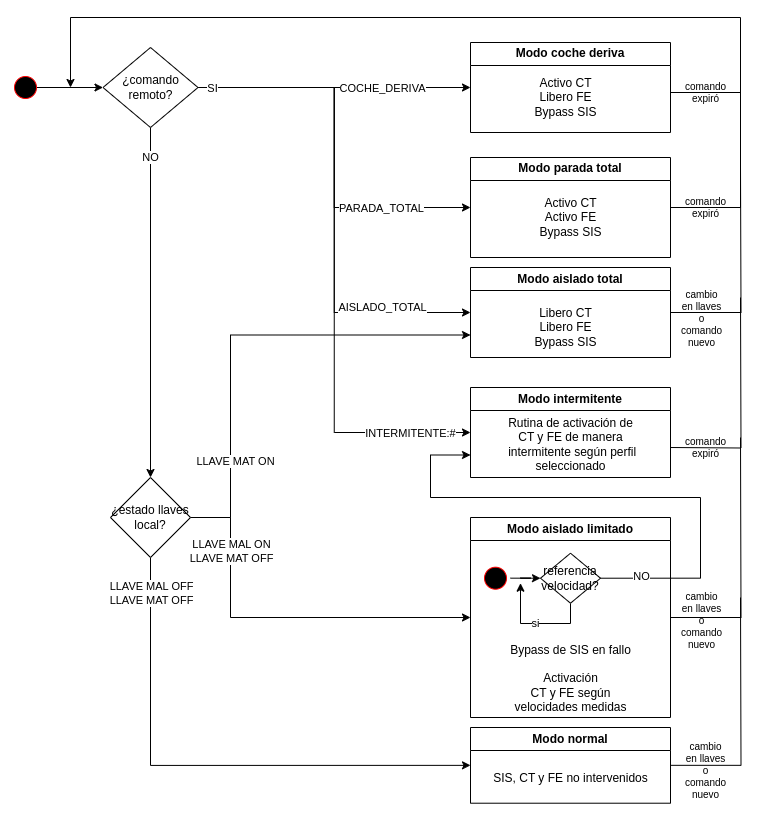
\includegraphics[width = \linewidth]{img/modos_salt.png}    
    \caption{Diagrama de flujo de modos de operación del SAL/T}
    \label{fig:modos_salt}
\end{figure}    
